% CREATED BY MAGNUS GUSTAVER, 2020
\chapter{Results}\label{results}

This chapter presents the results of the project. Primarily the result corresponding to the main aim of the project, meaning the bike's ability to balance, will be presented. The results correlating to the sub-goals: how the bike performs with regards to the steering motor, forward motor and balancing algorithm are also presented. Finally the reasons behind the results, and the effects of them are discussed. Further more detailed results from the individual tests are documented in appendix \ref{testingProtocol}.

\section{Steering Motor}

The steering motor, when viewed as a standalone component fully works as intended. That is, it is disabled until the \textit{GO} button is pressed in LabVIEW, and then it can be controlled by changing the duty cycle between 10\% and 90\%. It also stops when the duty cycle is set to 50\%, as expected. When the emergency stop is pressed either physically or in the software, the duty cycle is set to 50\%, and the pin is disabled. 

When connecting the control of the steering motor to the balancing algorithm and safety limit, the motor turns towards the same direction which the bike is leaning, and the duty cycle is set to 50\% when the safety limits is reached. However, the steering wheel has the possibility of overshooting the safety limit because of the inertia of the steering wheel and handlebar. Whether this happens also depends on how fast it was rotating before the limit was reached.

The controls for the motors, separated into two boxes are depicted in figure \ref{fig:motorControl} below. Inside of the left box, the steering motor controls are located. In these controls there exist inputs for changing each of the PID gains labeled P, I, and D. The box also has a field for changing the angle limit (in degrees from when the wheel is straight). Below the controls mentioned above are outputs from the steering motor encoder which shows its current position, velocity and acceleration. For the purpose of calibrating the encoder, there exists a button which resets the encoder position whenever it is pressed. At the bottom of the box, the duty cycle sent to the motor from the balancing algorithm is shown. At the bottom right of the image, under the boxes, is the \textit{GO} button which starts the two motors.

\begin{figure}[ht]
    \centering
    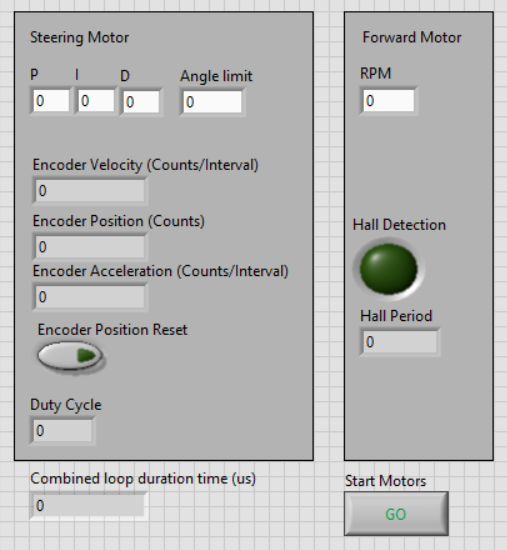
\includegraphics[width=7cm]{figure/motor_control.png}
    \caption{The motor controls in LabVIEW, with the steering motor control on the left side}
    \label{fig:motorControl}
\end{figure}

\section{Forward Motor}

The speed of the forward motor can successfully be set using the LabVIEW front panel as seen on the right side of figure \ref{fig:motorControl} above, and also changed while the program is running. The forward motor only starts when \textit{GO} is pressed, and it stops when the emergency stop is pressed; the same behavior that the steering motor has. 

The motor can not only be controlled by setting its speed directly, but also by changing its current. Controlling the motor using current can be accomplished if the function called by the \textit{Call Library Function Node} is changed to \texttt{setCurrent}. Additional methods of controlling the motor can be added by creating and calling additional C functions based on the example by Vedder.

\section{Balancing Algorithm} \label{results:balancing}

During the initial testing of the balancing algorithm, it was concluded that the steering motor behaved as expected in terms of rotation direction in relation to the roll rate of the bike. Meaning when the bike was leaned, the front wheel rotated towards the same direction. 

When the bike was then placed on the roller, it seemed as if the bike could stay upright for some time before it had to be caught to prevent it from falling. The algorithm would make the front wheel rotate to the correct direction, but the amplitude of these rotations was gradually increasing until the border of the roller was reached. A real, conclusive result could not be made from this test; the reasons for this are both because of human interference, as well as the narrow width of the roller.

The final and most reliable test of the balancing algorithm was done outdoors as described in \ref{method:unaidedTest}, and the P gain was set to 5 (I and D were set to 0). The data from these tests, recorded with the logging system, are presented in the images below.

\begin{figure}[H]
    \begin{subfigure}{.5\textwidth}
        \centering
        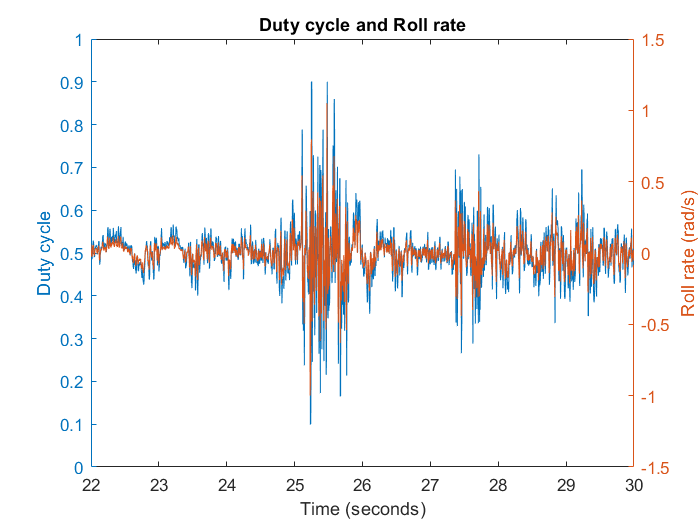
\includegraphics[width=\textwidth]{figure/dutyAndRoll.png}
        \caption{The roll rate of the bike and duty cycle sent from the balancing algorithm.}
        \label{fig:dutyAndRoll}
    \end{subfigure}
    \begin{subfigure}{.5\textwidth}
        \centering
        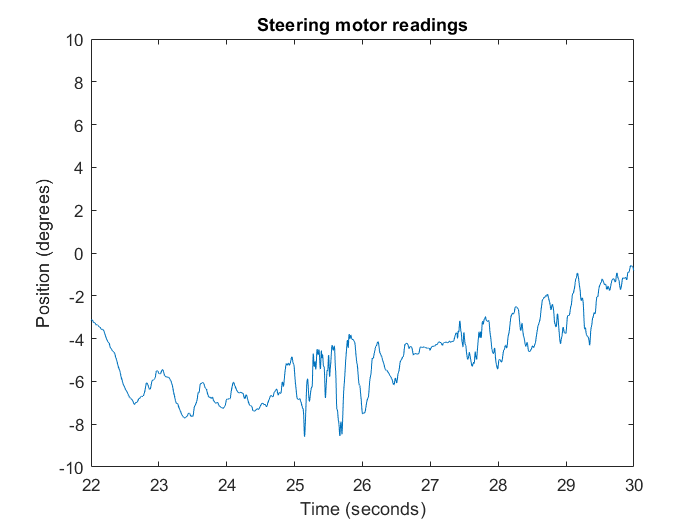
\includegraphics[width=\textwidth]{figure/motorPosition.png}
        \caption{The position of steering motor during the test.}
        \label{fig:motorPosition}
    \end{subfigure}
\caption{Plotted data from the final test.}
\label{fig:finalTest}
\end{figure}

In the test presented above the roll rate of the bike is relatively stable around 0. There only major deviance is around the 25:th second, which is caused by the bike passing over a bump in the road. As seen in blue line in figure \ref{fig:dutyAndRoll} which represents the duty cycle, the rapid change in duty cycle also leads to a change by the control algorithm as a correction. The steering motor has some oscillations with and amplitude of about $2\degree$ and period of roughly one second. That is however nothing which had any noticeable effect on the overall performance; the test lasted for 8 seconds, and had to be aborted when the bike drove too close to obstacles in the testing area.

\section{Loop Times}

For the loop time tests all of the bikes hardware was enabled so that all control signal calculations would be made, and the resulting time would be as accurate possible. The total loop time was recorded as being between \SI{2155}{\micro\second} and \SI{2420}{\micro\second}. Compared to the previous project group's measurements, the new loop times are at worst is \SI{240}{\micro\second} slower than the worst case before the logging system and C algorithms were added \cite{AronssonKarlsson2022PROJECTAUTOBIKE}.

\section{Discussion} \label{results:discussion}

The main part of the result which should be discussed is that the forward motor control stopped working before the final test. Meaning that the UART commands sent to the VESC did not result in the forward motor moving. The reasons for this are unknown, but the problem has been isolated to the VESC, perhaps a broken trace related to the UART connections are the cause. During the final test the bike was instead accelerated by pushing it, before being let go. Pushing the bike should though not affect the overall result, compared to if the forward motor was still working.

The improvement of the development experience is one aim which was presented in \ref{intro:aim}, this aim is however not mentioned above. The reason being this decision it that it is difficult to assess if the aim has been reached or not, since it can be considered individual to a certain degree. What can be said is that all of the code which is used has been moved to a single location, which should make it easier to find the code. It should also now be much clearer what code is the most recent one. The code itself has been organized and separated into sub-VIs which should also make it easier to find the relevant code, this in combination with more comments should also make it easier to understand it.

What the result of the final test, and the data in figure \ref{fig:finalTest} shows is that the bike can be kept stable by the balancing algorithm, even when the surface is uneven. There are some low frequency osculations of about the same frequency in all of the plotted data, which indicates that primarily the P gain of the PID controller could be tuned for better results.

There are some high frequency oscillations in the roll rate which might be caused by the IMU not being properly mounted, something which leads to vibrations; especially when the surface is uneven. Improper mounting of hardware can also be found elsewhere in the bike, which could be contributing to a worse balancing performance. These oscillations also creates high frequency changes in the duty cycle. Though this is generally not a problem since the steering wheel cannot change direction with such a high frequency; the dynamics of the bike could be described as acting as a low pass filter.
